% \documentclass[dvipdfmx, 11pt]{beamer}
\documentclass[aspectratio=169, dvipdfmx, 11pt]{beamer} % aspectratio=43, 149, 169
\usepackage{here, amsmath, latexsym, amssymb, bm, ascmac, mathtools, multicol, tcolorbox, subfig}

%デザインの選択(省略可)
\usetheme{Luebeck}
%カラーテーマの選択(省略可)
\usecolortheme{orchid}
%フォントテーマの選択(省略可)
\usefonttheme{professionalfonts}
%フレーム内のテーマの選択(省略可)
\useinnertheme{circles}
%フレーム外側のテーマの選択(省略可)
\useoutertheme{infolines}
%しおりの文字化け解消
\usepackage{atbegshi}
\ifnum 42146=\euc"A4A2
\AtBeginShipoutFirst{\special{pdf:tounicode EUC-UCS2}}
\else
\AtBeginShipoutFirst{\special{pdf:tounicode 90ms-RKSJ-UCS2}}
\fi
%ナビゲーションバー非表示
\setbeamertemplate{navigation symbols}{}
%既定をゴシック体に
\renewcommand{\kanjifamilydefault}{\gtdefault}
%タイトル色
\setbeamercolor{title}{fg=structure, bg=}
%フレームタイトル色
\setbeamercolor{frametitle}{fg=structure, bg=}
%スライド番号のみ表示
%\setbeamertemplate{footline}[frame number]
%itemize
\setbeamertemplate{itemize item}{\small\raise0.5pt\hbox{$\bullet$}}
\setbeamertemplate{itemize subitem}{\tiny\raise1.5pt\hbox{$\blacktriangleright$}}
\setbeamertemplate{itemize subsubitem}{\tiny\raise1.5pt\hbox{$\bigstar$}}
% color
\newcommand{\red}[1]{\textcolor{red}{#1}}
\newcommand{\green}[1]{\textcolor{green!40!black}{#1}}
\newcommand{\blue}[1]{\textcolor{blue!80!black}{#1}}

\title[凸解析学における漸近挙動]{凸解析学における漸近挙動}
\subtitle{Introduction of Asymptotic Cones}
\author[岩本 崚汰]{岩本 崚汰}
\institute[新潟大学大学院]{新潟大学大学院自然科学研究科}
\date{March 14, 2023}

\begin{document}
\maketitle

\begin{frame}{目次}
    \tableofcontents
\end{frame}

\section{前提条件 (Precondition) }
\begin{frame}{目次}
    \tableofcontents[currentsection]
\end{frame}

\begin{frame}{前提条件 (Precondition) }

  今回扱うのは $\mathbb{R}^n$ の実ベクトル空間とする。

  また、内積は以下のように定義する。

  \begin{equation}
    \text{For}\: x=(x_1,\dots,x_n) \in \mathbb{R}^n \:\text{and}\: y=(y_1,\dots,y_n) \in \mathbb{R}^n, \left\langle x,y\right\rangle \coloneqq \sum_{i = 1}^{n} x_i y_i. \notag
  \end{equation}

  ノルムに関しては、$\left\lVert x \right\rVert \coloneqq \left\langle x,x\right\rangle ^{1/2} $ とする。

\end{frame}

\section{錐 (Cones) }
\begin{frame}{目次}
  \tableofcontents[currentsection]
\end{frame}

\begin{frame}{錐 (Cones) }
  \begin{description}
    \item[(1)] 錐の定義
    \item[(2)] 錐の特徴付け(凸解析学で登場する様々な錐の紹介)
  \end{description}
\end{frame}

\begin{frame}{錐の定義 (1) }
  \begin{block}{定義 2.1}
    $C \subset \mathbb{R}^n$, $C \neq \varnothing$ とする。以下を満たすときに $C$ は \textit{cone} であるという。

    \begin{equation}
      \forall x \in C, t \geq 0, tx \in C. \notag
    \end{equation}

  \end{block}
  \centering
  \begin{columns}
    \begin{column}{0.31\textwidth}
      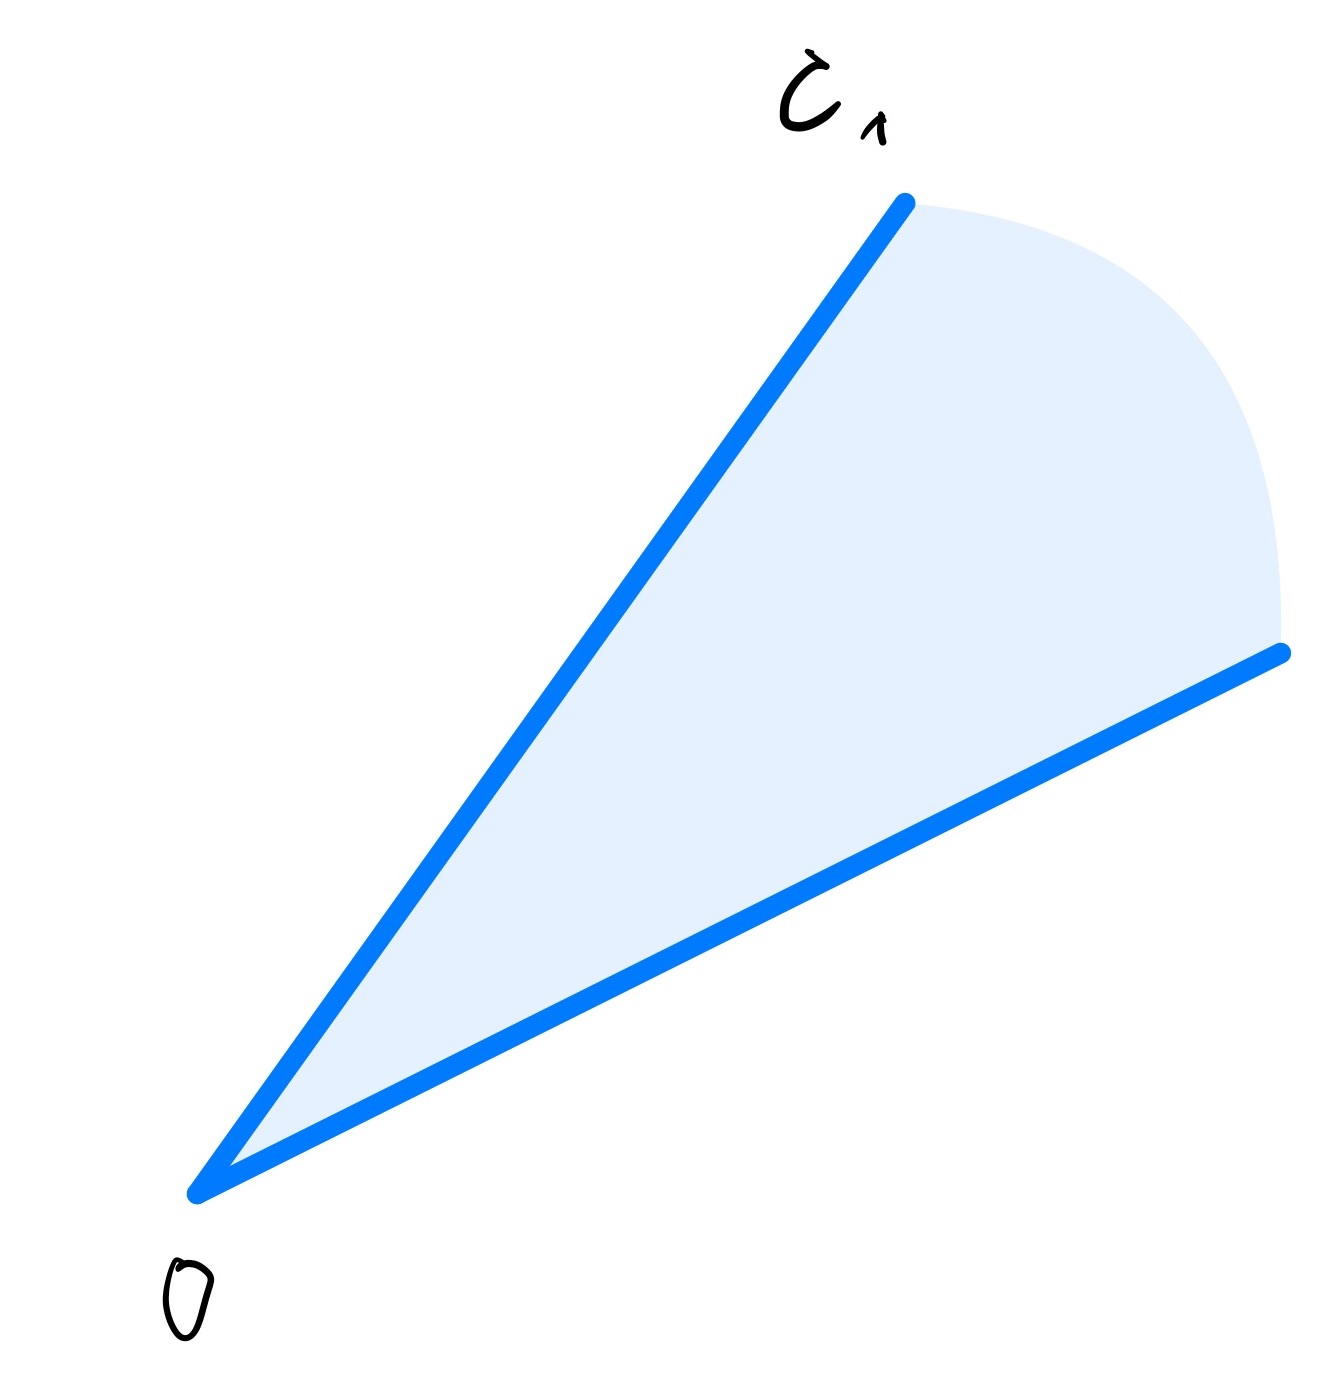
\includegraphics[keepaspectratio, scale=0.08]{figures/cone_figure_1.jpg}
    \end{column}
    \begin{column}{0.31\textwidth}
      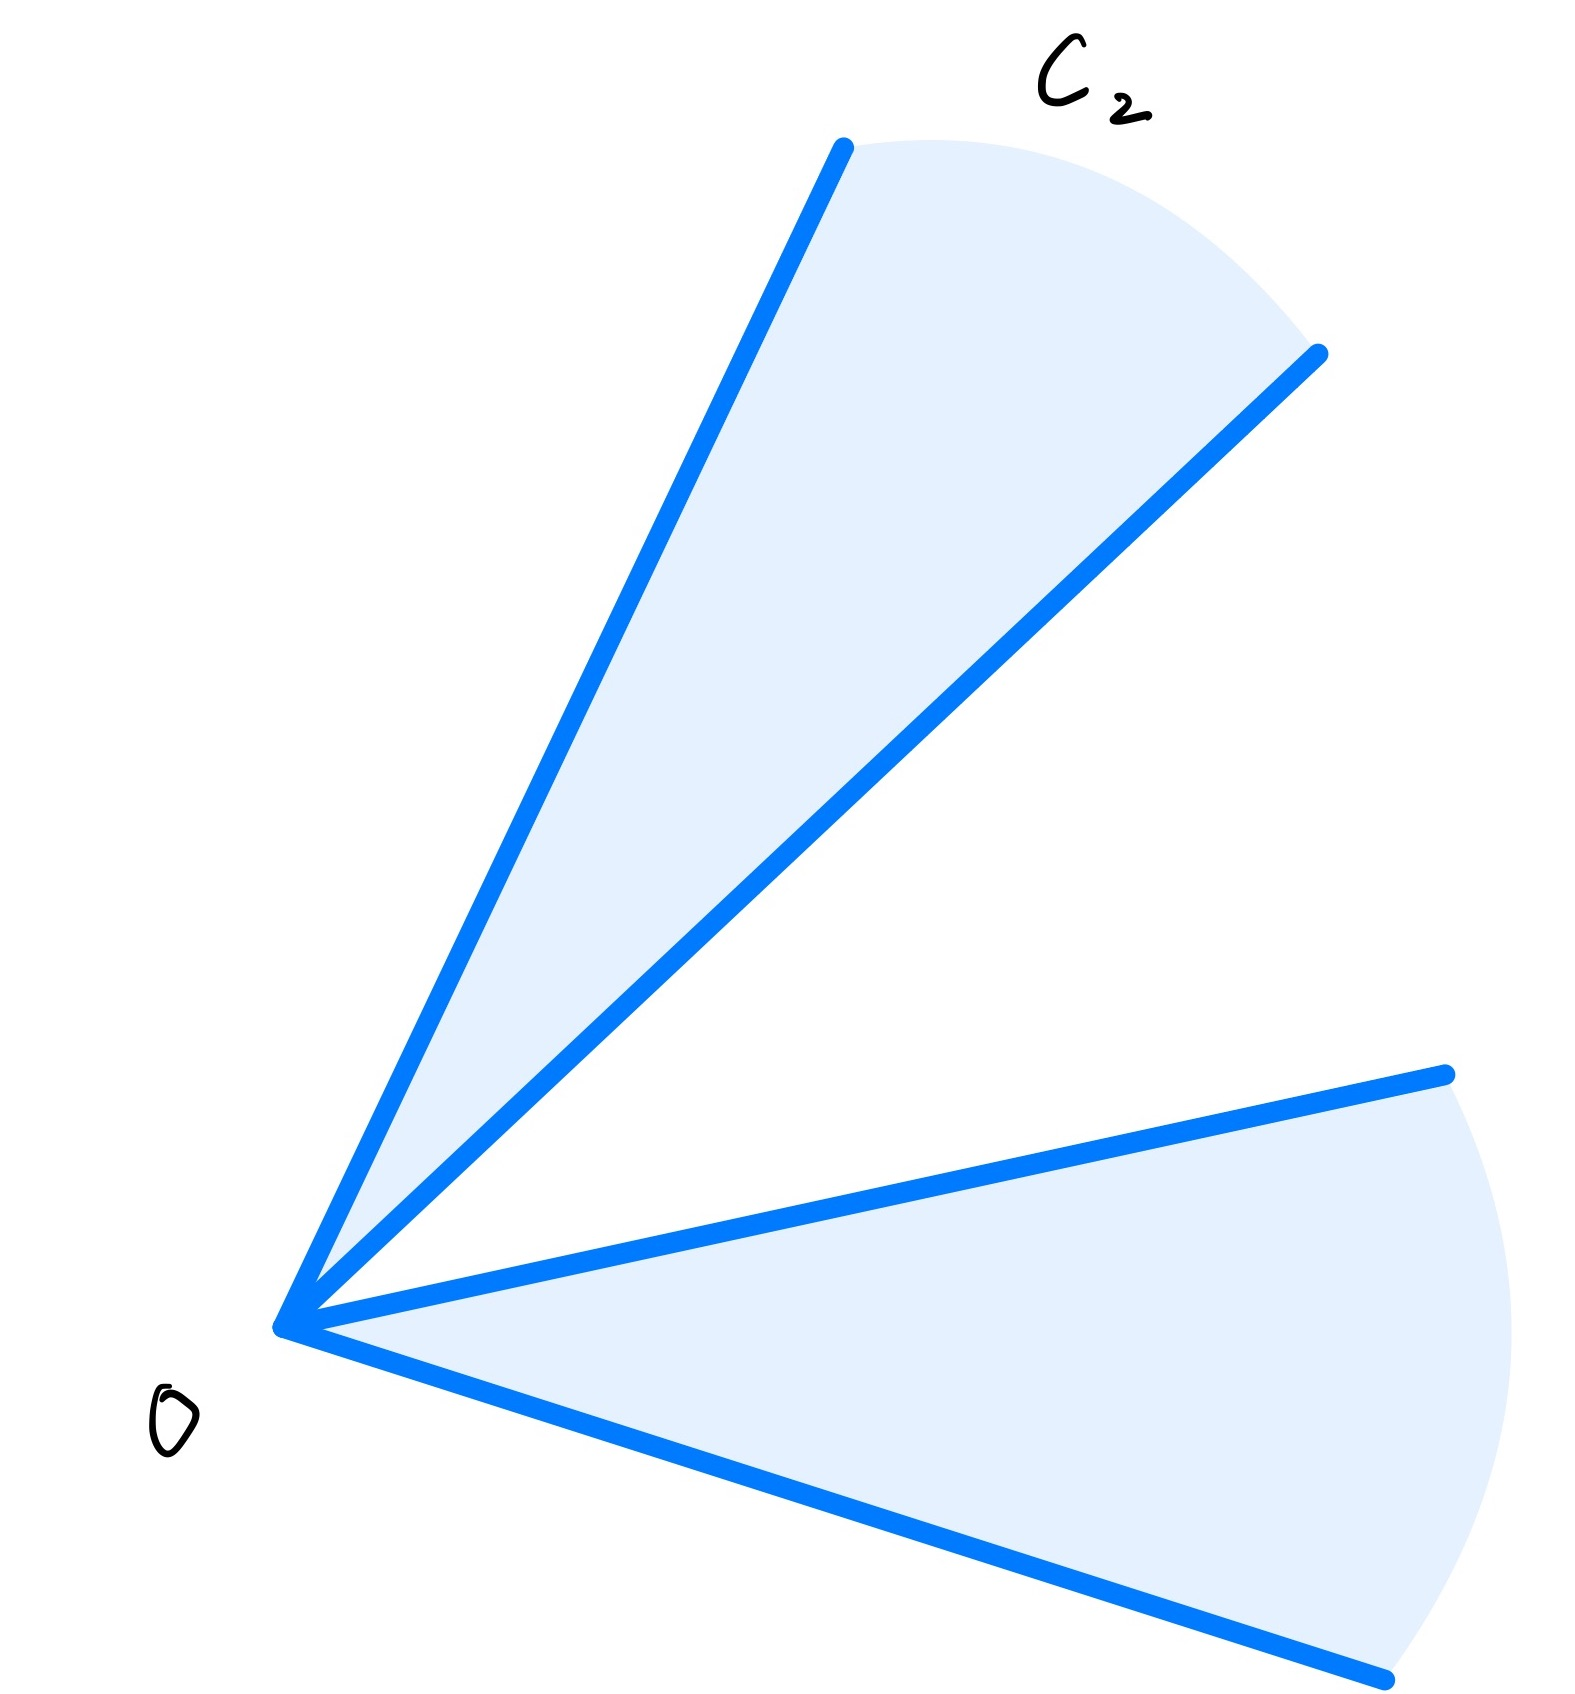
\includegraphics[keepaspectratio, scale=0.06]{figures/cone_figure_2.jpg}
    \end{column}
    \begin{column}{0.31\textwidth}
      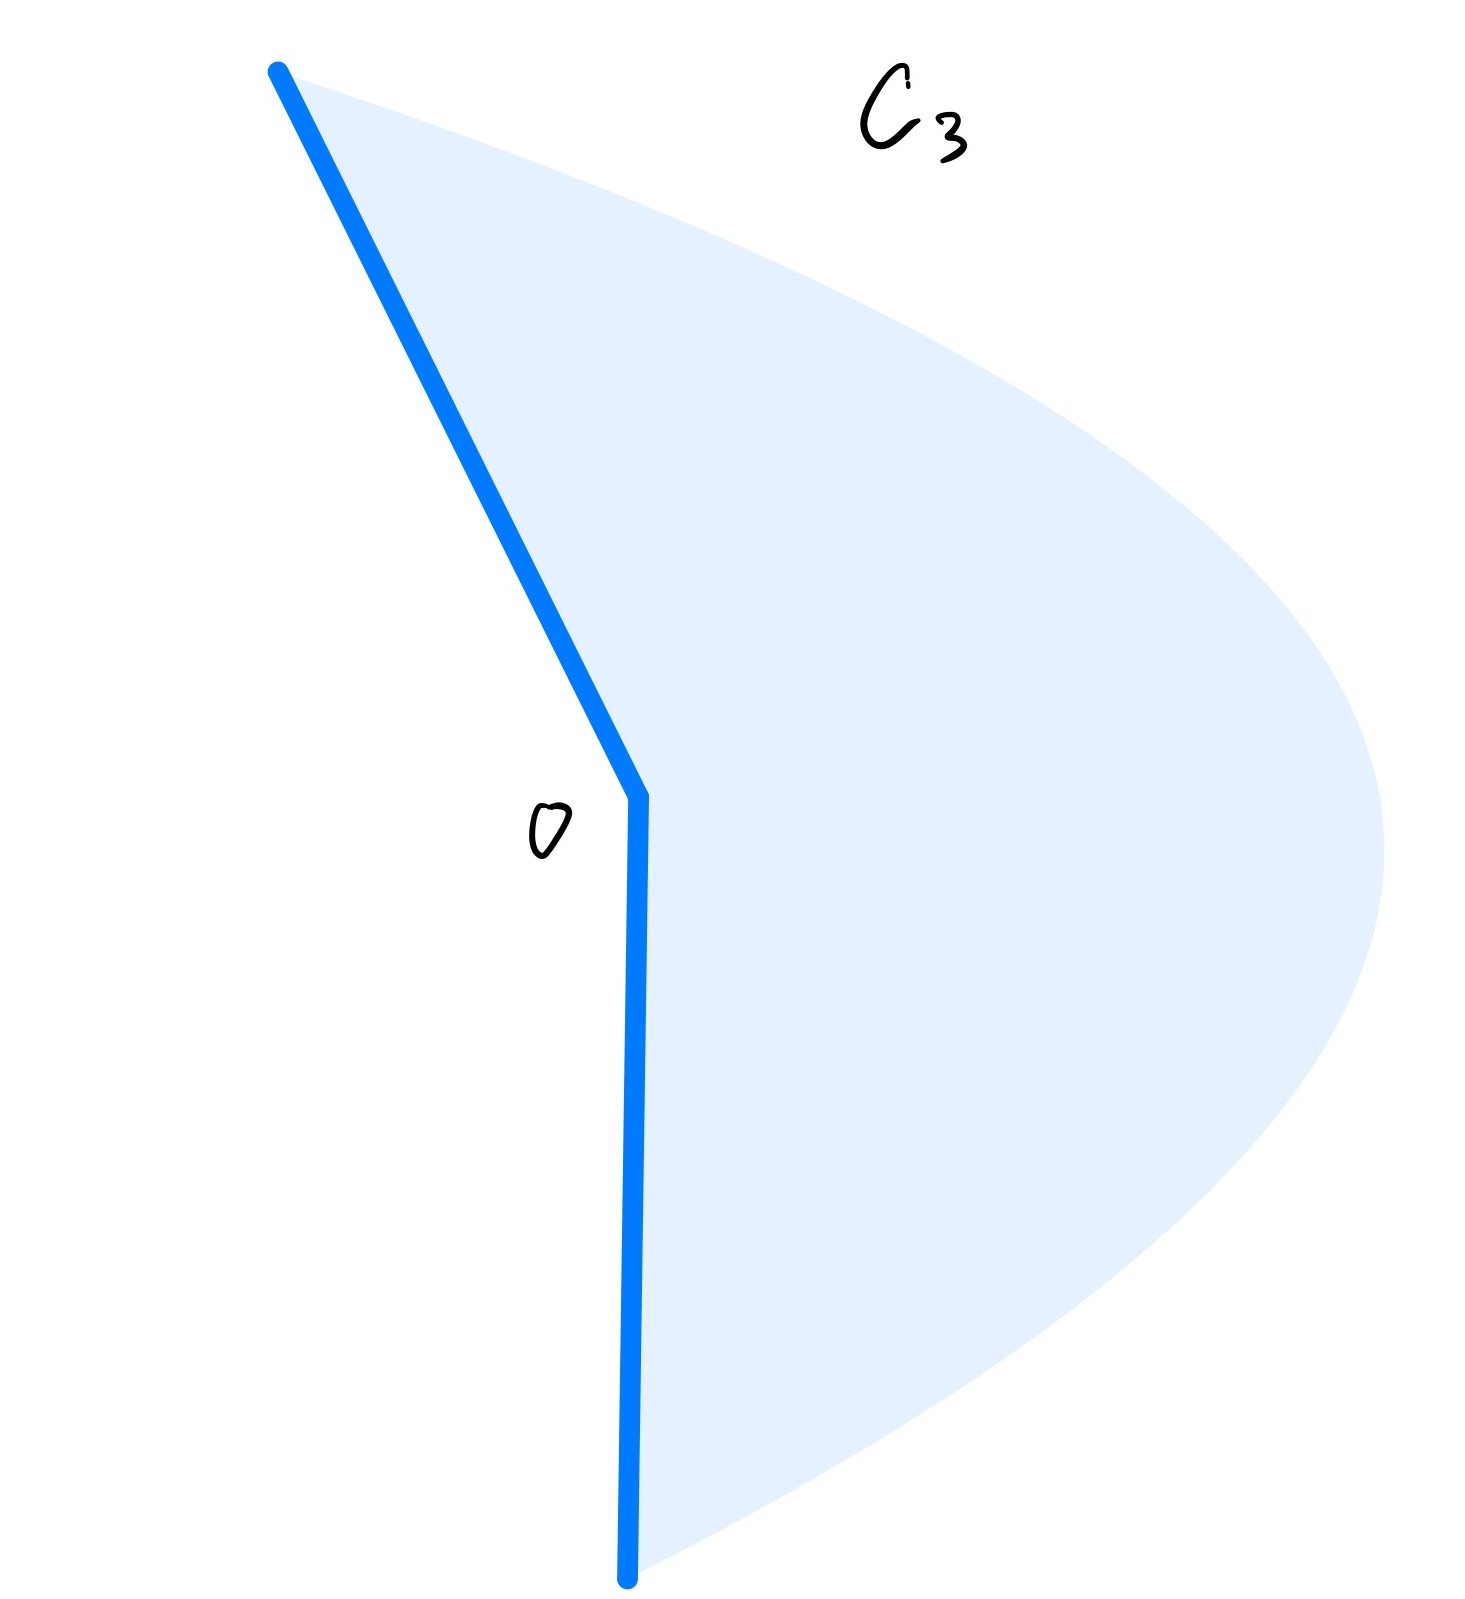
\includegraphics[keepaspectratio, scale=0.06]{figures/cone_figure_3.jpg}
    \end{column}
\end{columns}

\end{frame}

\begin{frame}{錐の定義 (2) }
  \begin{block}{命題 2.2}
    $C \subset \mathbb{R}^n$, $C \neq \varnothing$ とする。このとき以下の命題は同値である。

    (a) $C$ は凸錐である。

    (b) $C$ は $C + C \subset C$ を満たす錐である。

  \end{block}

  \centering
  \begin{columns}
    \begin{column}{0.48\textwidth}
      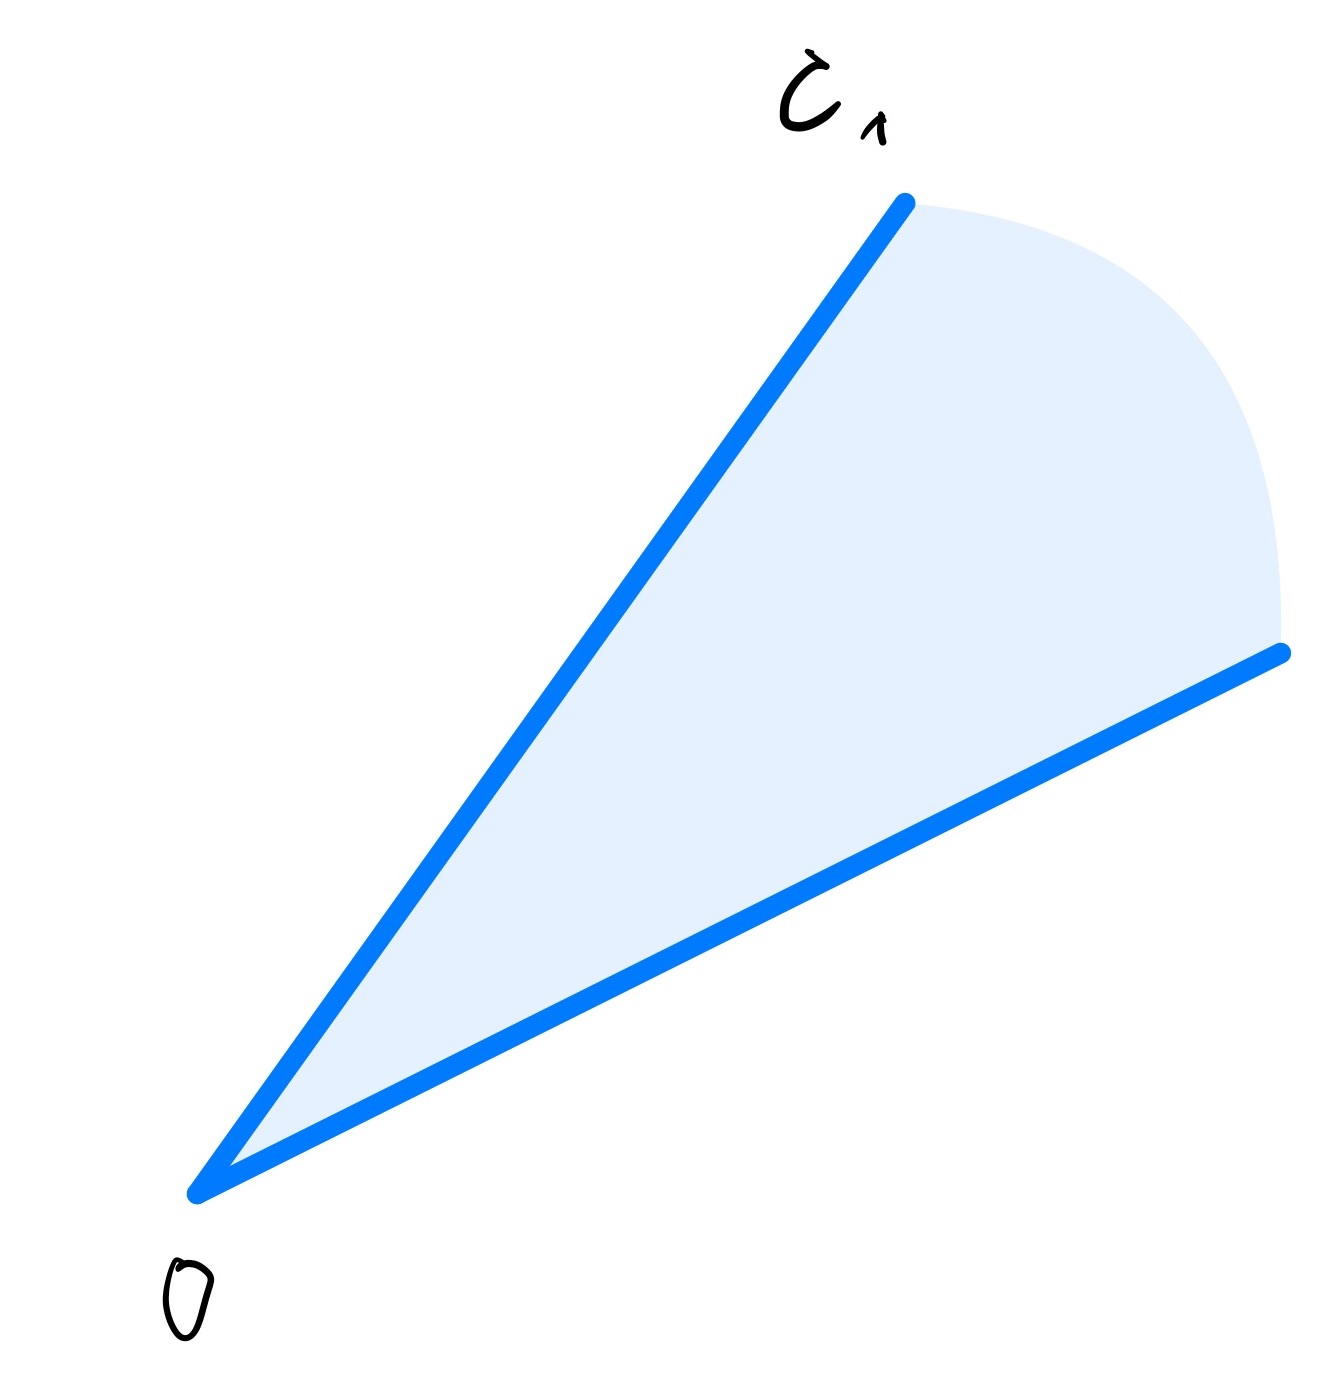
\includegraphics[keepaspectratio, scale=0.08]{figures/cone_figure_1.jpg}
    \end{column}
    \begin{column}{0.48\textwidth}
      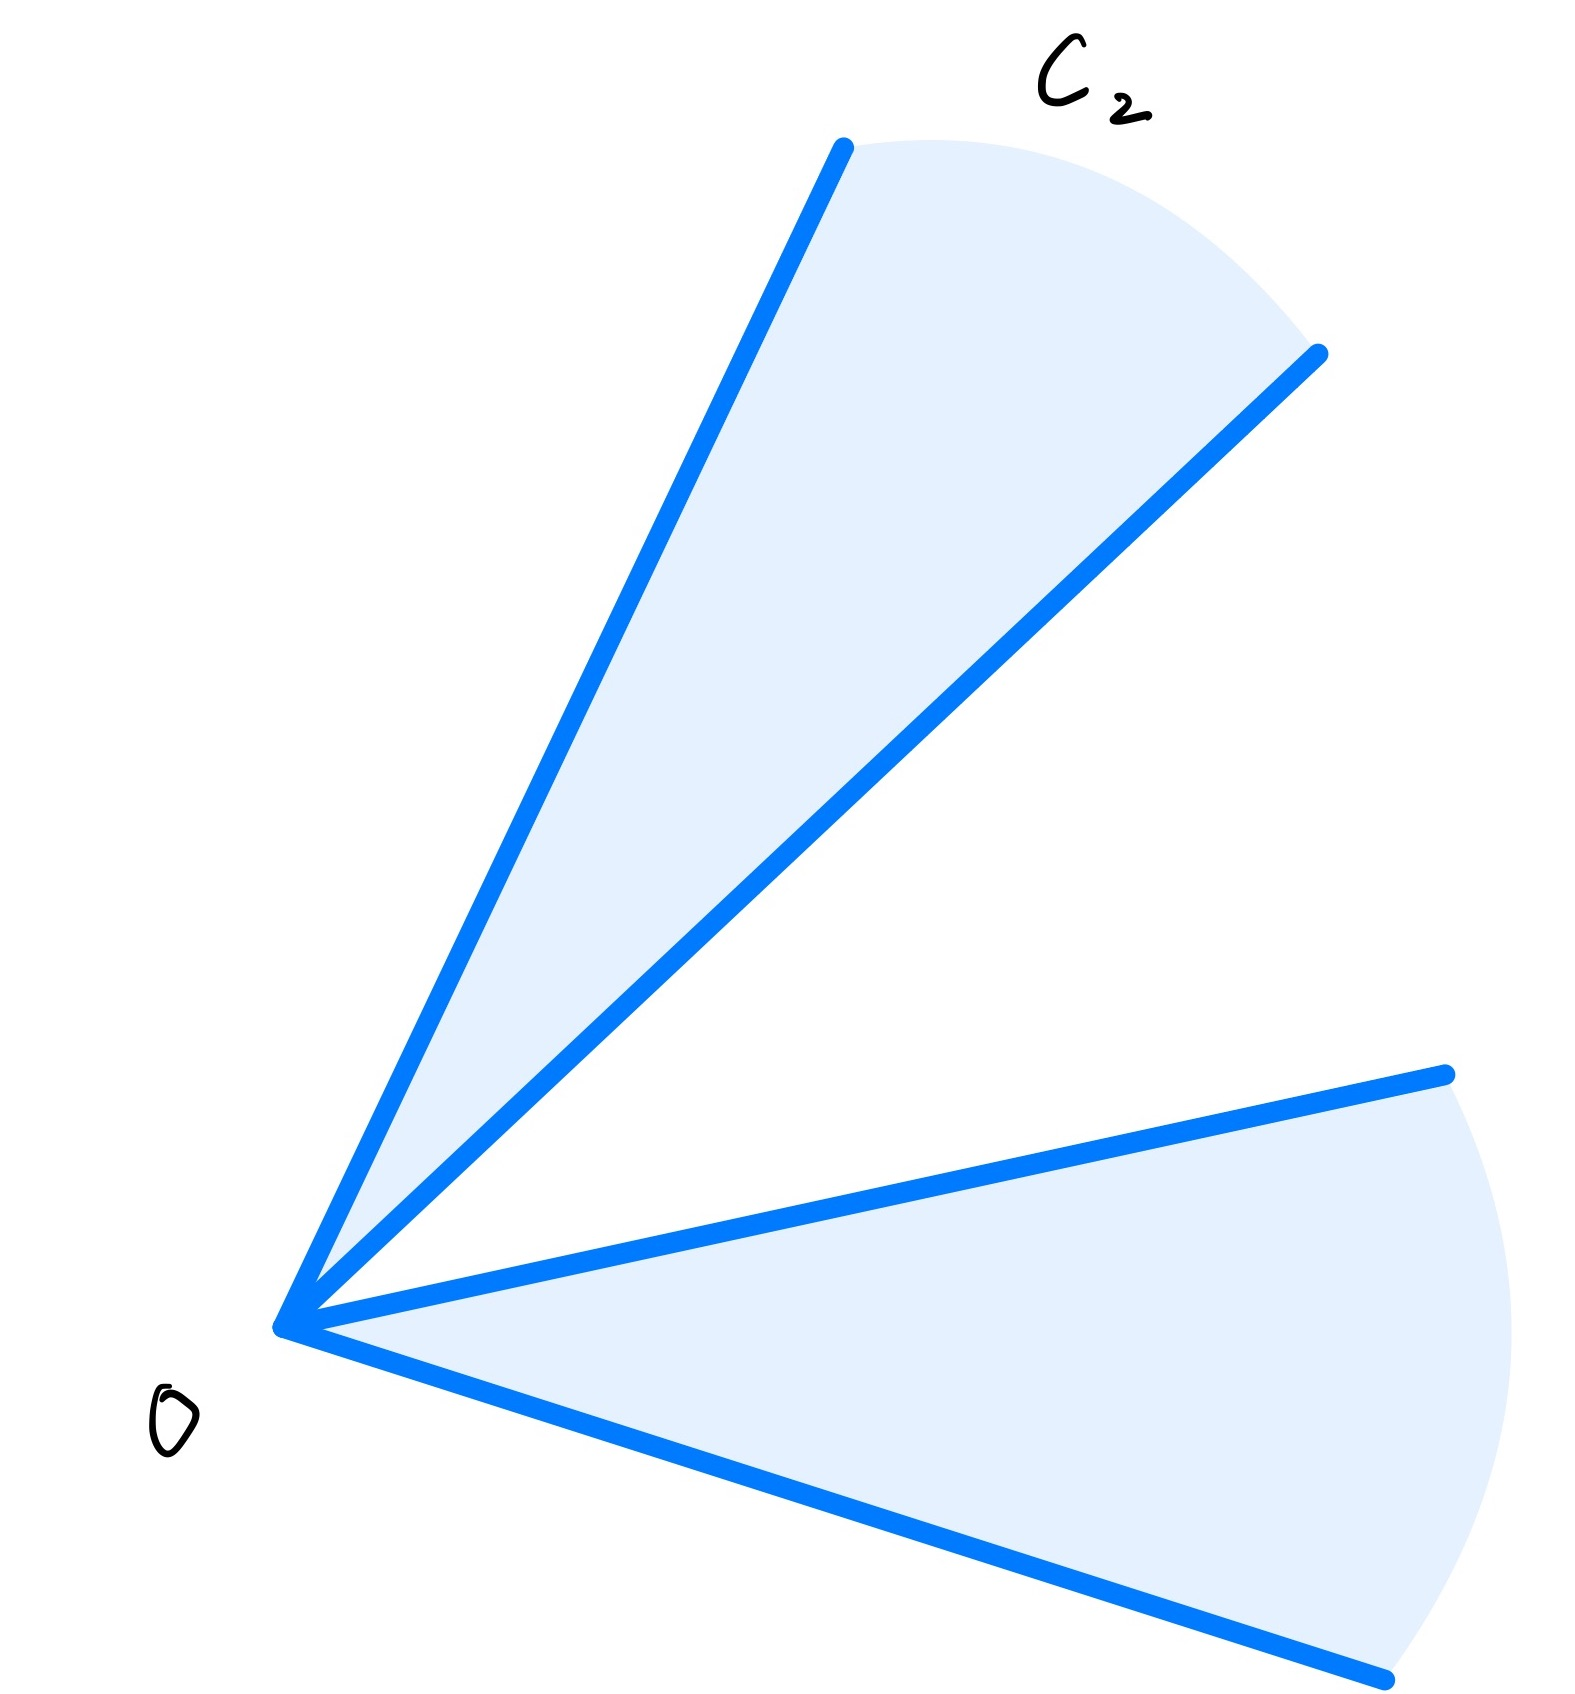
\includegraphics[keepaspectratio, scale=0.06]{figures/cone_figure_2.jpg}
    \end{column}
  \end{columns}
\end{frame}

\begin{frame}{錐の特徴付け (1)}
  \begin{block}{定義 2.3 (pointed) }
    $C \subset \mathbb{R}^n$, $C$ は錐であるとする。以下を満たすときに $C$ は \textit{pointed} であるという。

    \begin{equation}
      C \cap  (-C) = \{0\}. \notag
    \end{equation}

  \end{block}

  \centering
  \begin{columns}
    \begin{column}{0.48\textwidth}
      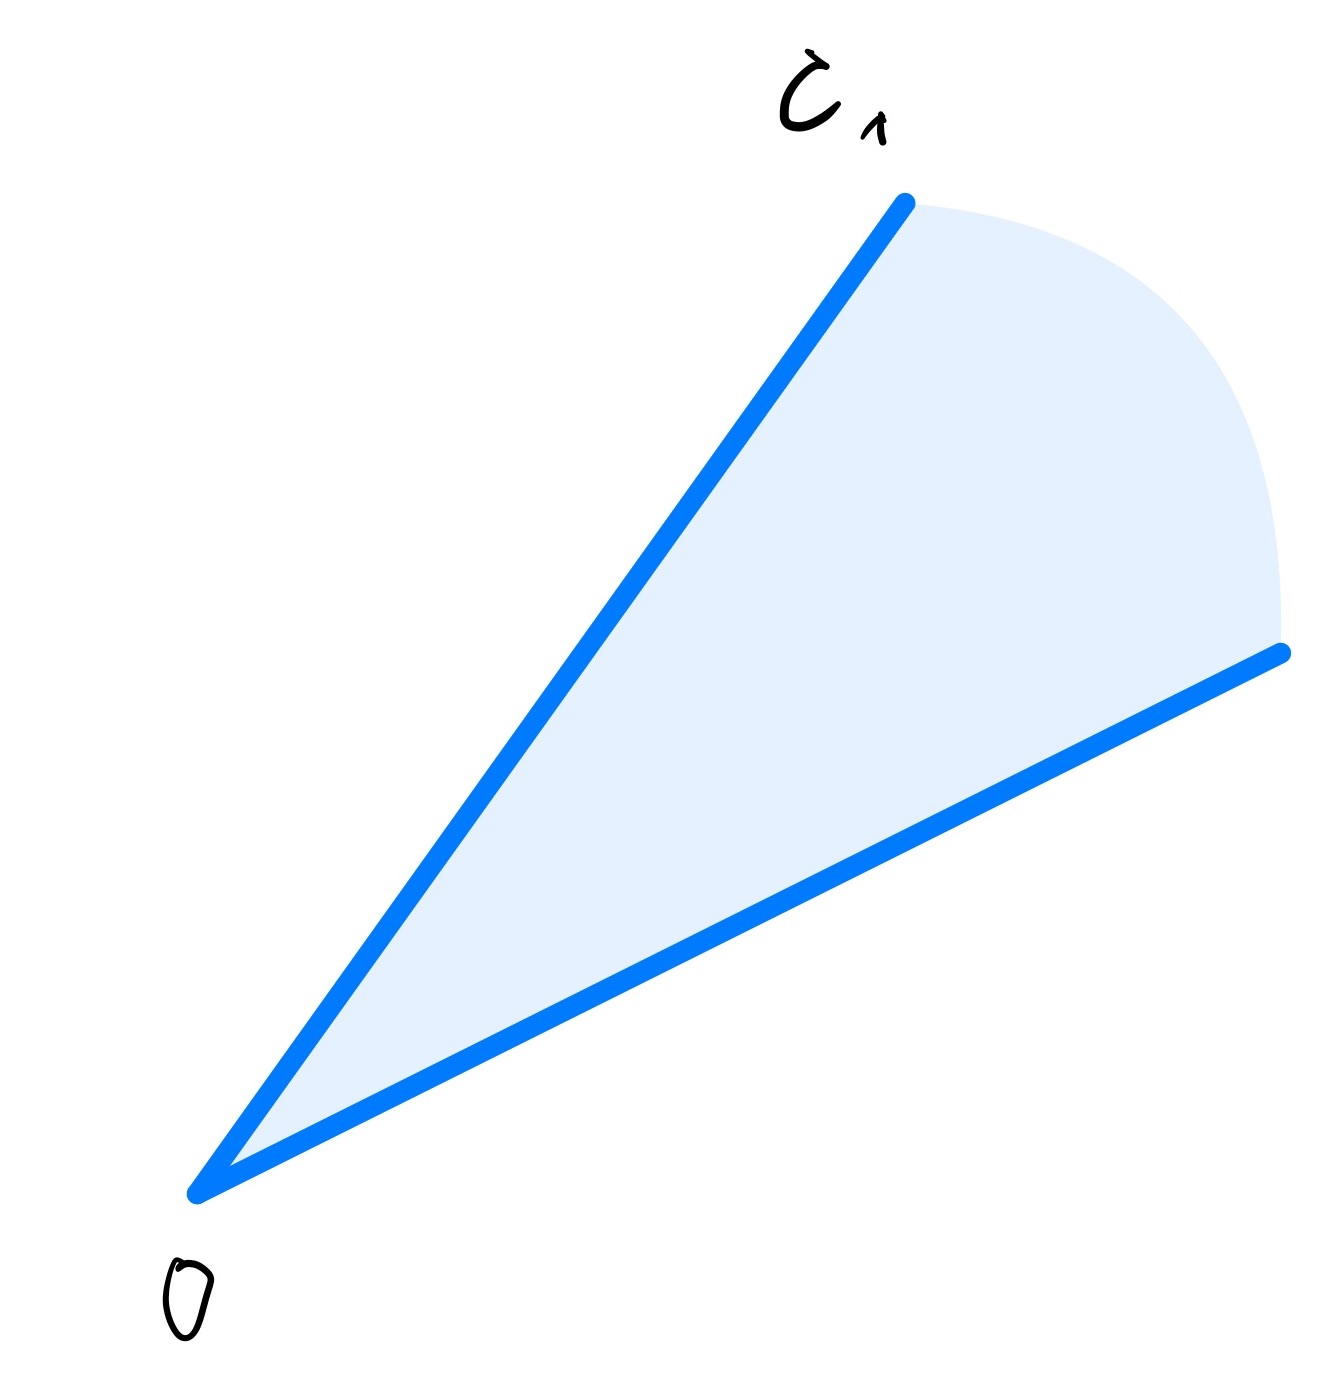
\includegraphics[keepaspectratio, scale=0.08]{figures/cone_figure_1.jpg}
    \end{column}
    \begin{column}{0.48\textwidth}
      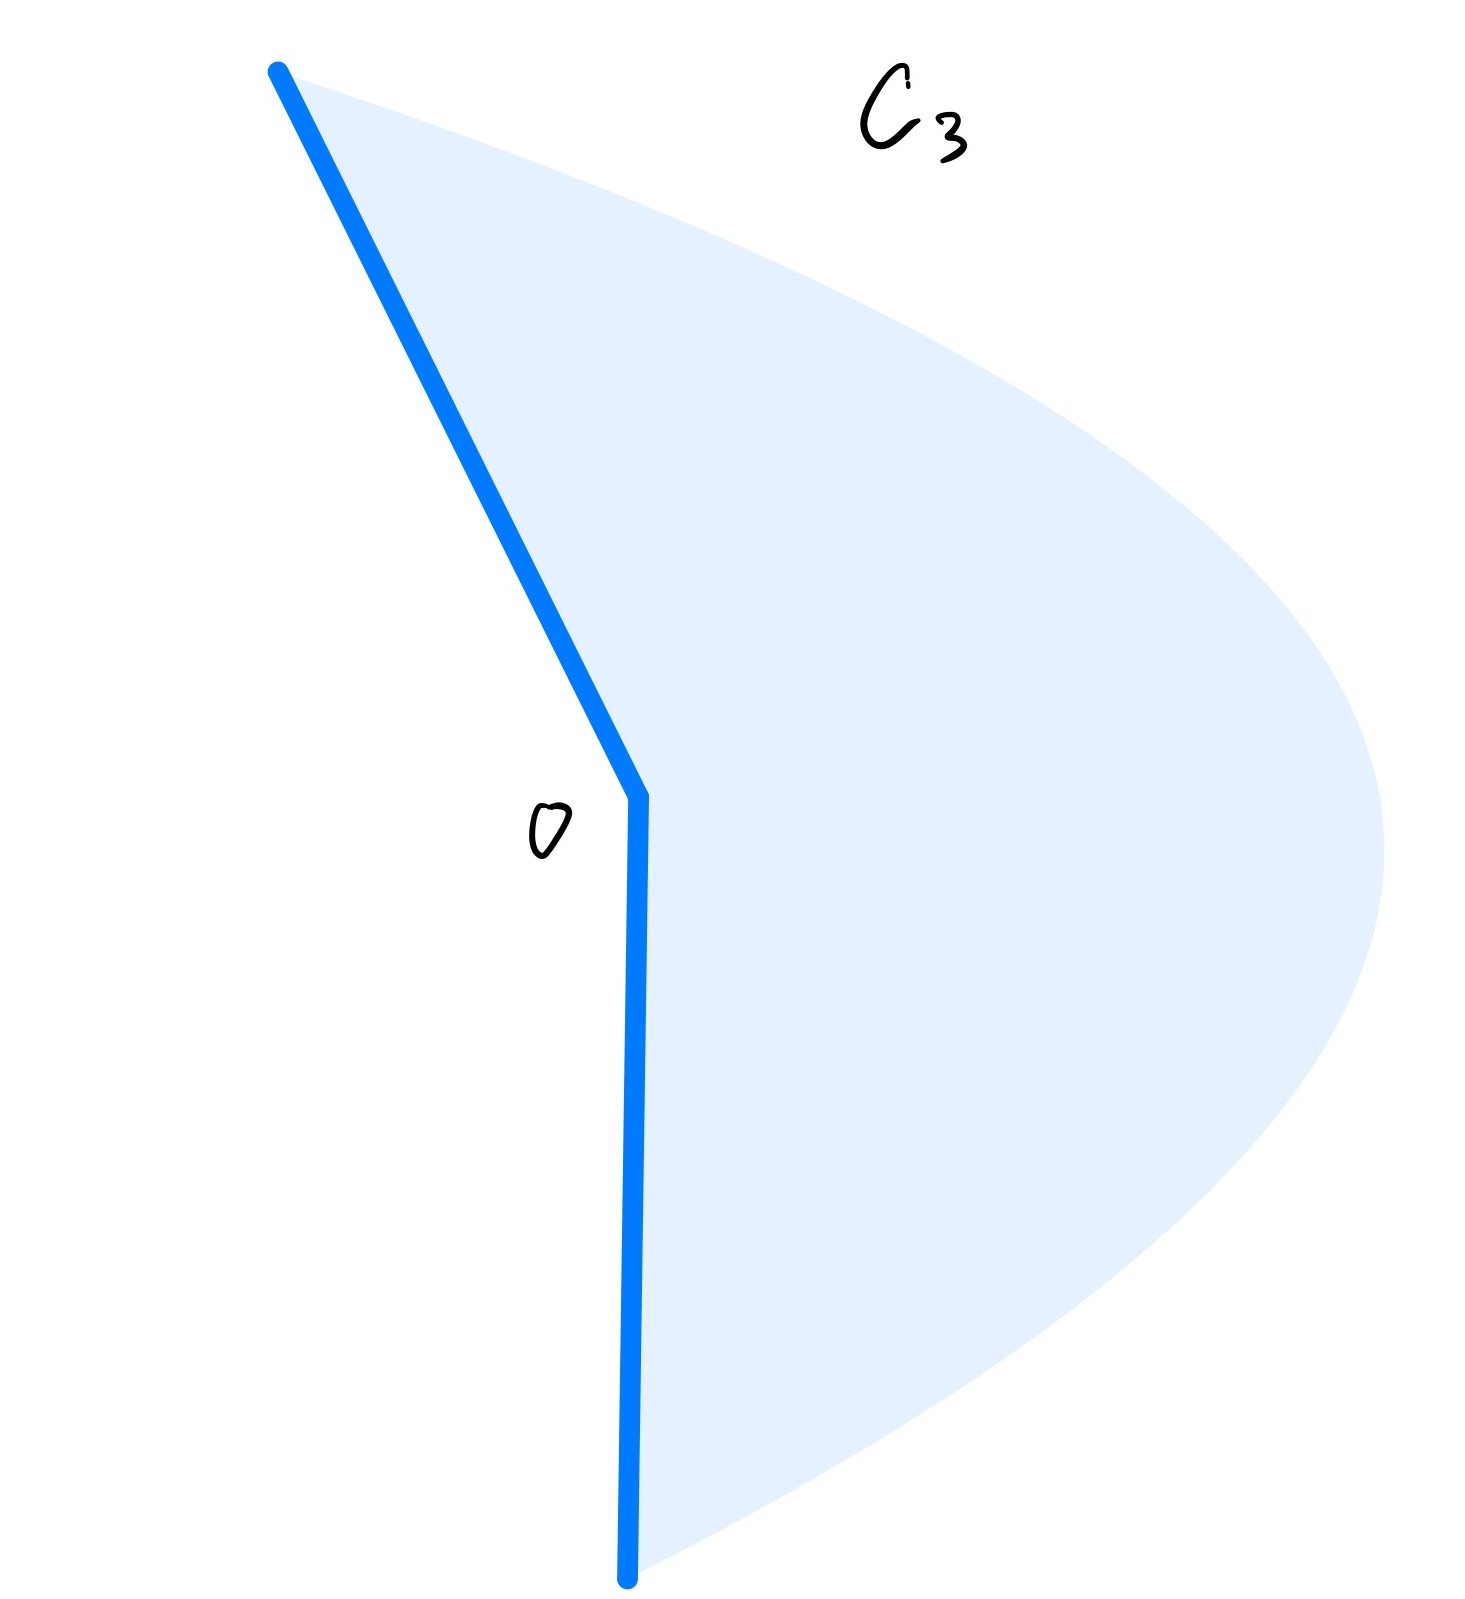
\includegraphics[keepaspectratio, scale=0.06]{figures/cone_figure_3.jpg}
    \end{column}
  \end{columns}
\end{frame}

\begin{frame}{錐の特徴付け (2)}
  \begin{block}{定義 2.4 (polar cone) }
    $C \subset \mathbb{R}^n$, $C$ は錐であるとする。このとき $C$ の極錐、$C^*$ は以下のように定義する。

    \begin{equation}
      C^* \coloneqq \{y \in \mathbb{R}^n \:|\: \left\langle y,x \right\rangle \leq 0 , \forall x \in C \}. \notag
    \end{equation}

  \end{block}
  \centering
  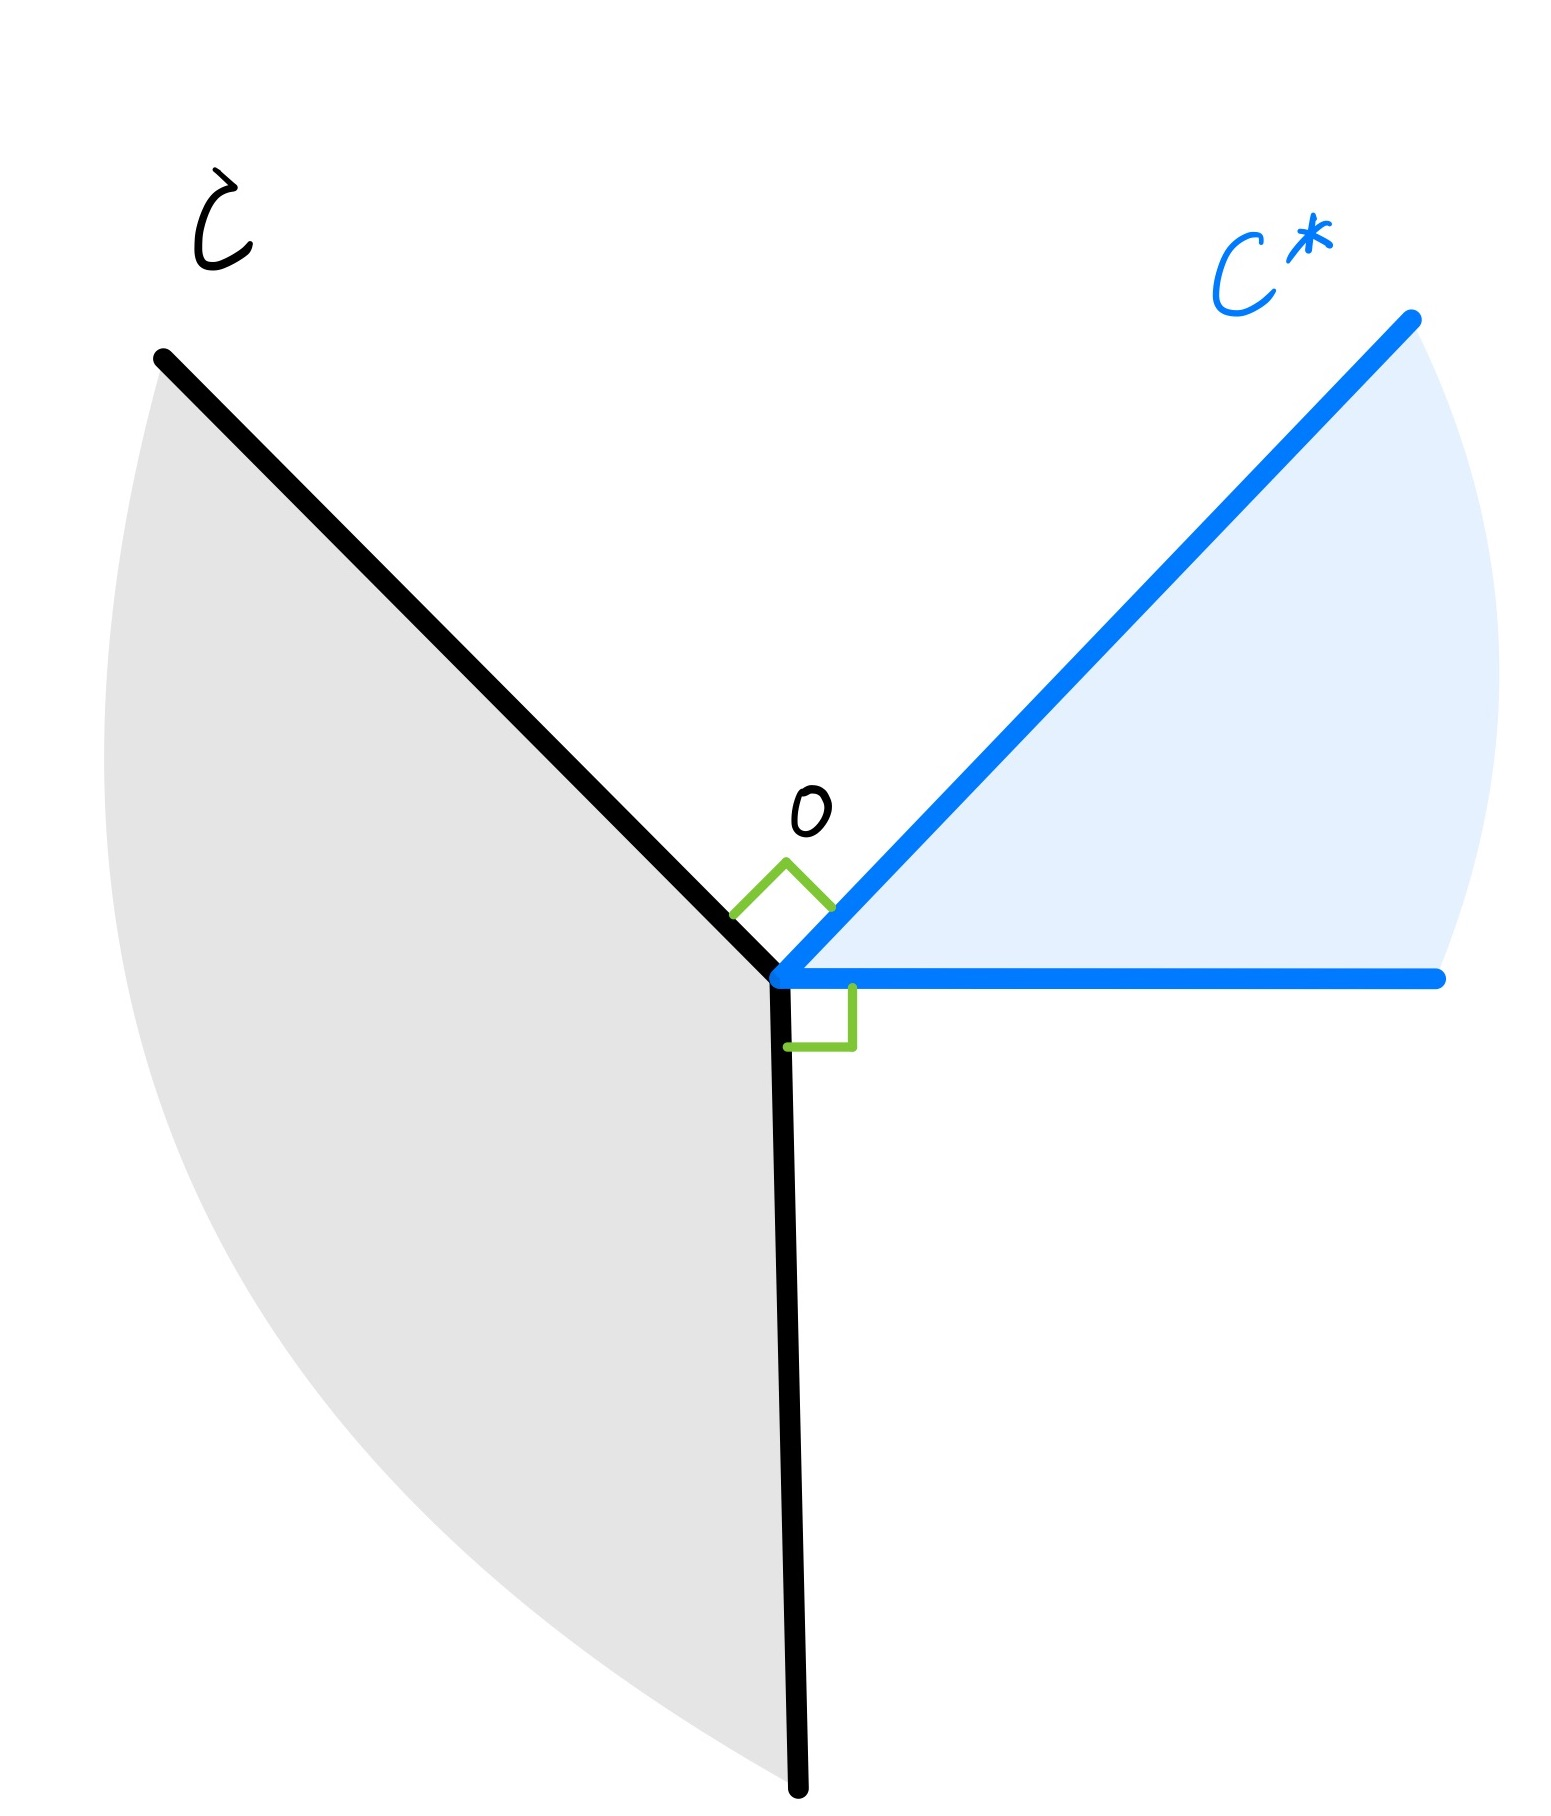
\includegraphics[keepaspectratio, scale=0.06]{figures/polar_cone.jpg}
\end{frame}

\begin{frame}{錐の特徴付け (3)}
  \begin{block}{定義 2.5 (normal cone) }
    $C \subset \mathbb{R}^n$, $C$ は空でない凸集合とし、$\bar{x} \in C$ とする。このとき $C$ の $\bar{x}$ での法錐、$N_C(\bar{x})$ は以下のように定義する。

    \begin{equation}
      N_C(\bar{x}) \coloneqq \{ v \in \mathbb{R}^n \:|\: \left\langle v, x - \bar{x} \right\rangle \leq 0, \forall x \in C \}. \notag
    \end{equation}

  \end{block}

  \centering
  \begin{columns}
    \begin{column}{0.48\textwidth}
      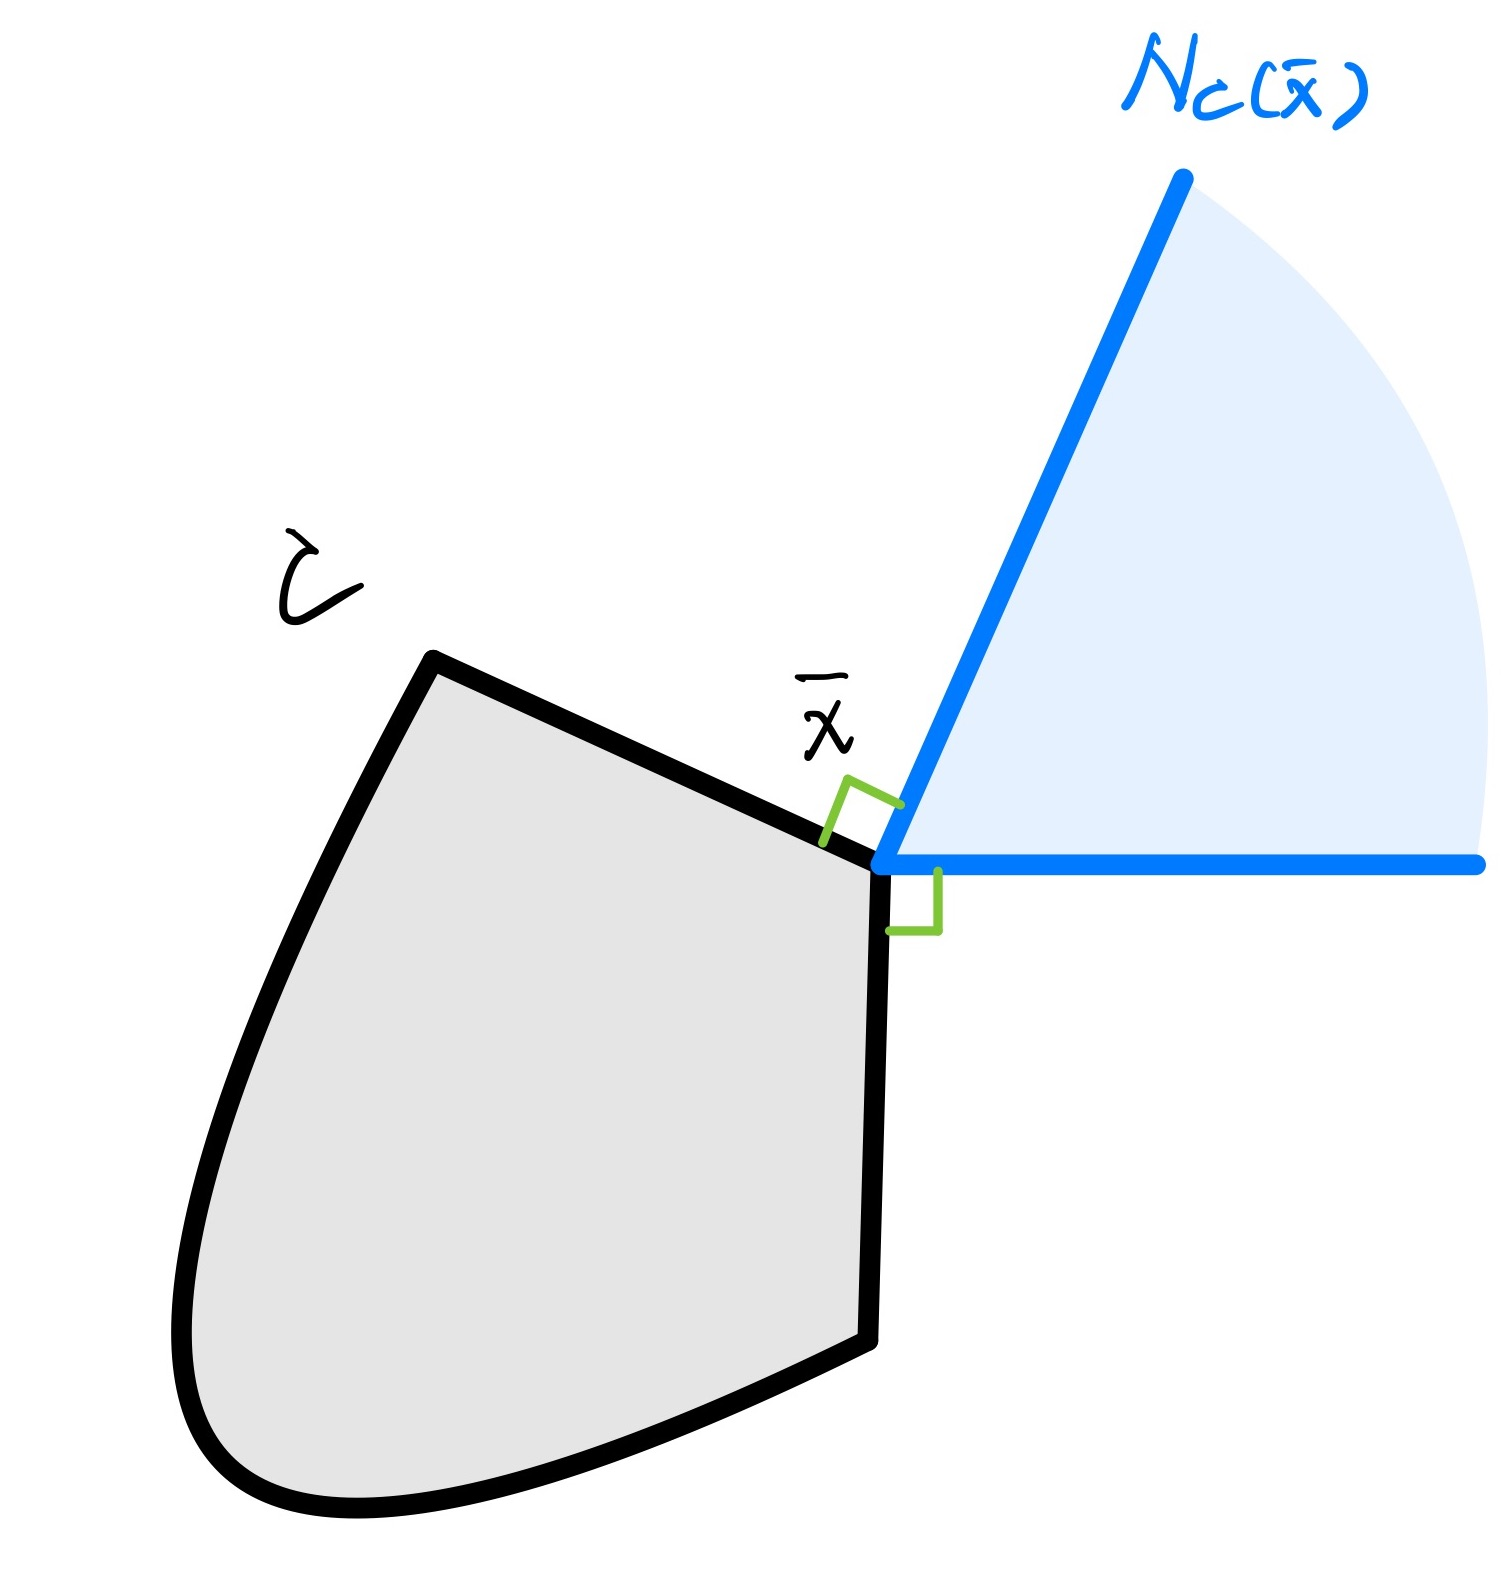
\includegraphics[keepaspectratio, scale=0.06]{figures/normal_cone_1.jpg}
    \end{column}
    \begin{column}{0.48\textwidth}
      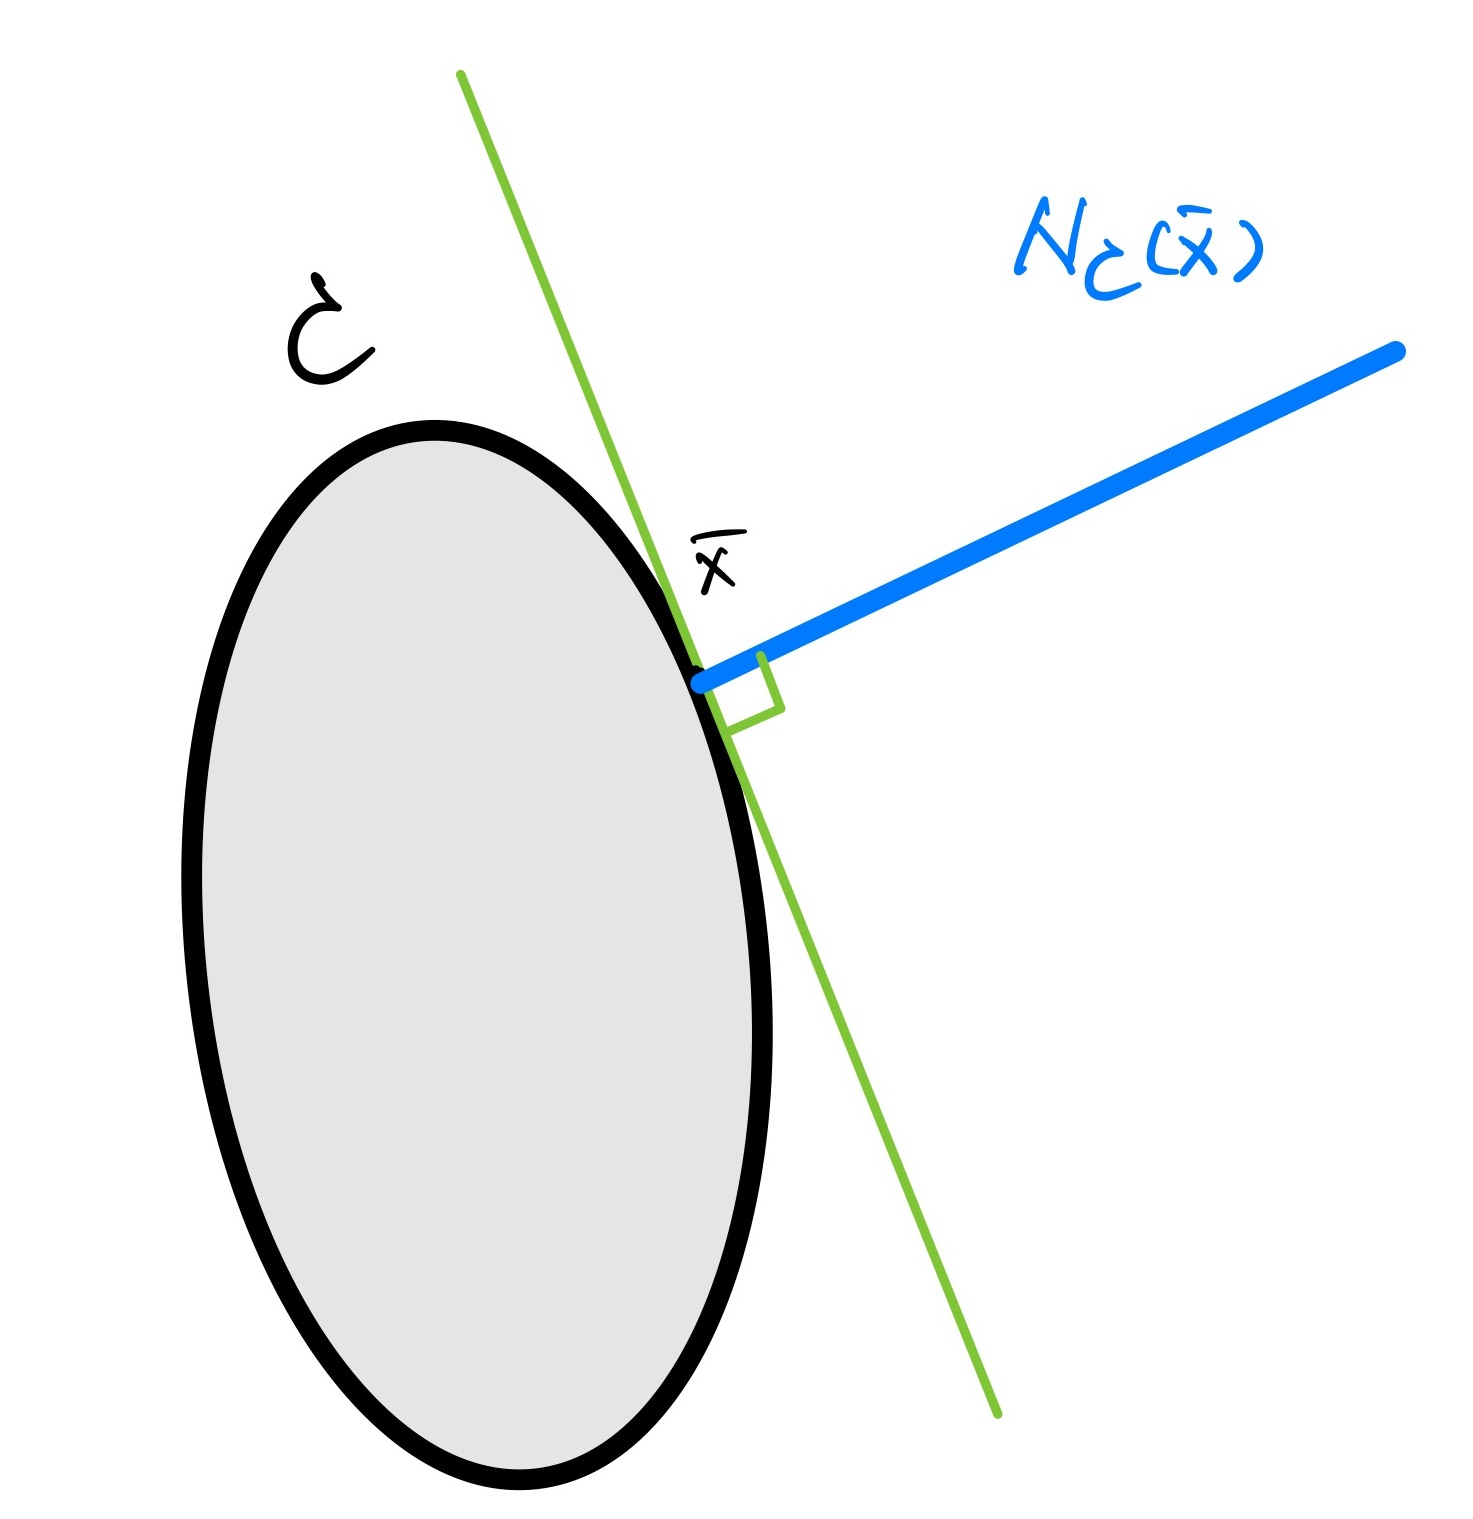
\includegraphics[keepaspectratio, scale=0.06]{figures/normal_cone_2.jpg}
    \end{column}
  \end{columns}
\end{frame}

\begin{frame}{錐の特徴付け (4)}
  \begin{block}{定義 2.6 (tangent cone) }
    $C \subset \mathbb{R}^n$, $C$ は空でない凸集合とし、$\bar{x} \in \text{cl}C$ とする。このとき $C$ の $\bar{x}$ での接錐、$T_C(\bar{x})$ は以下のように定義する。

    \begin{equation}
      T_C(\bar{x}) \coloneqq \text{cl}\{ d \in \mathbb{R}^n \:|\: \exists t > 0, \:with\: \bar{x} + td \in C \}. \notag
    \end{equation}

  \end{block}

  \centering
  \begin{columns}
    \begin{column}{0.48\textwidth}
      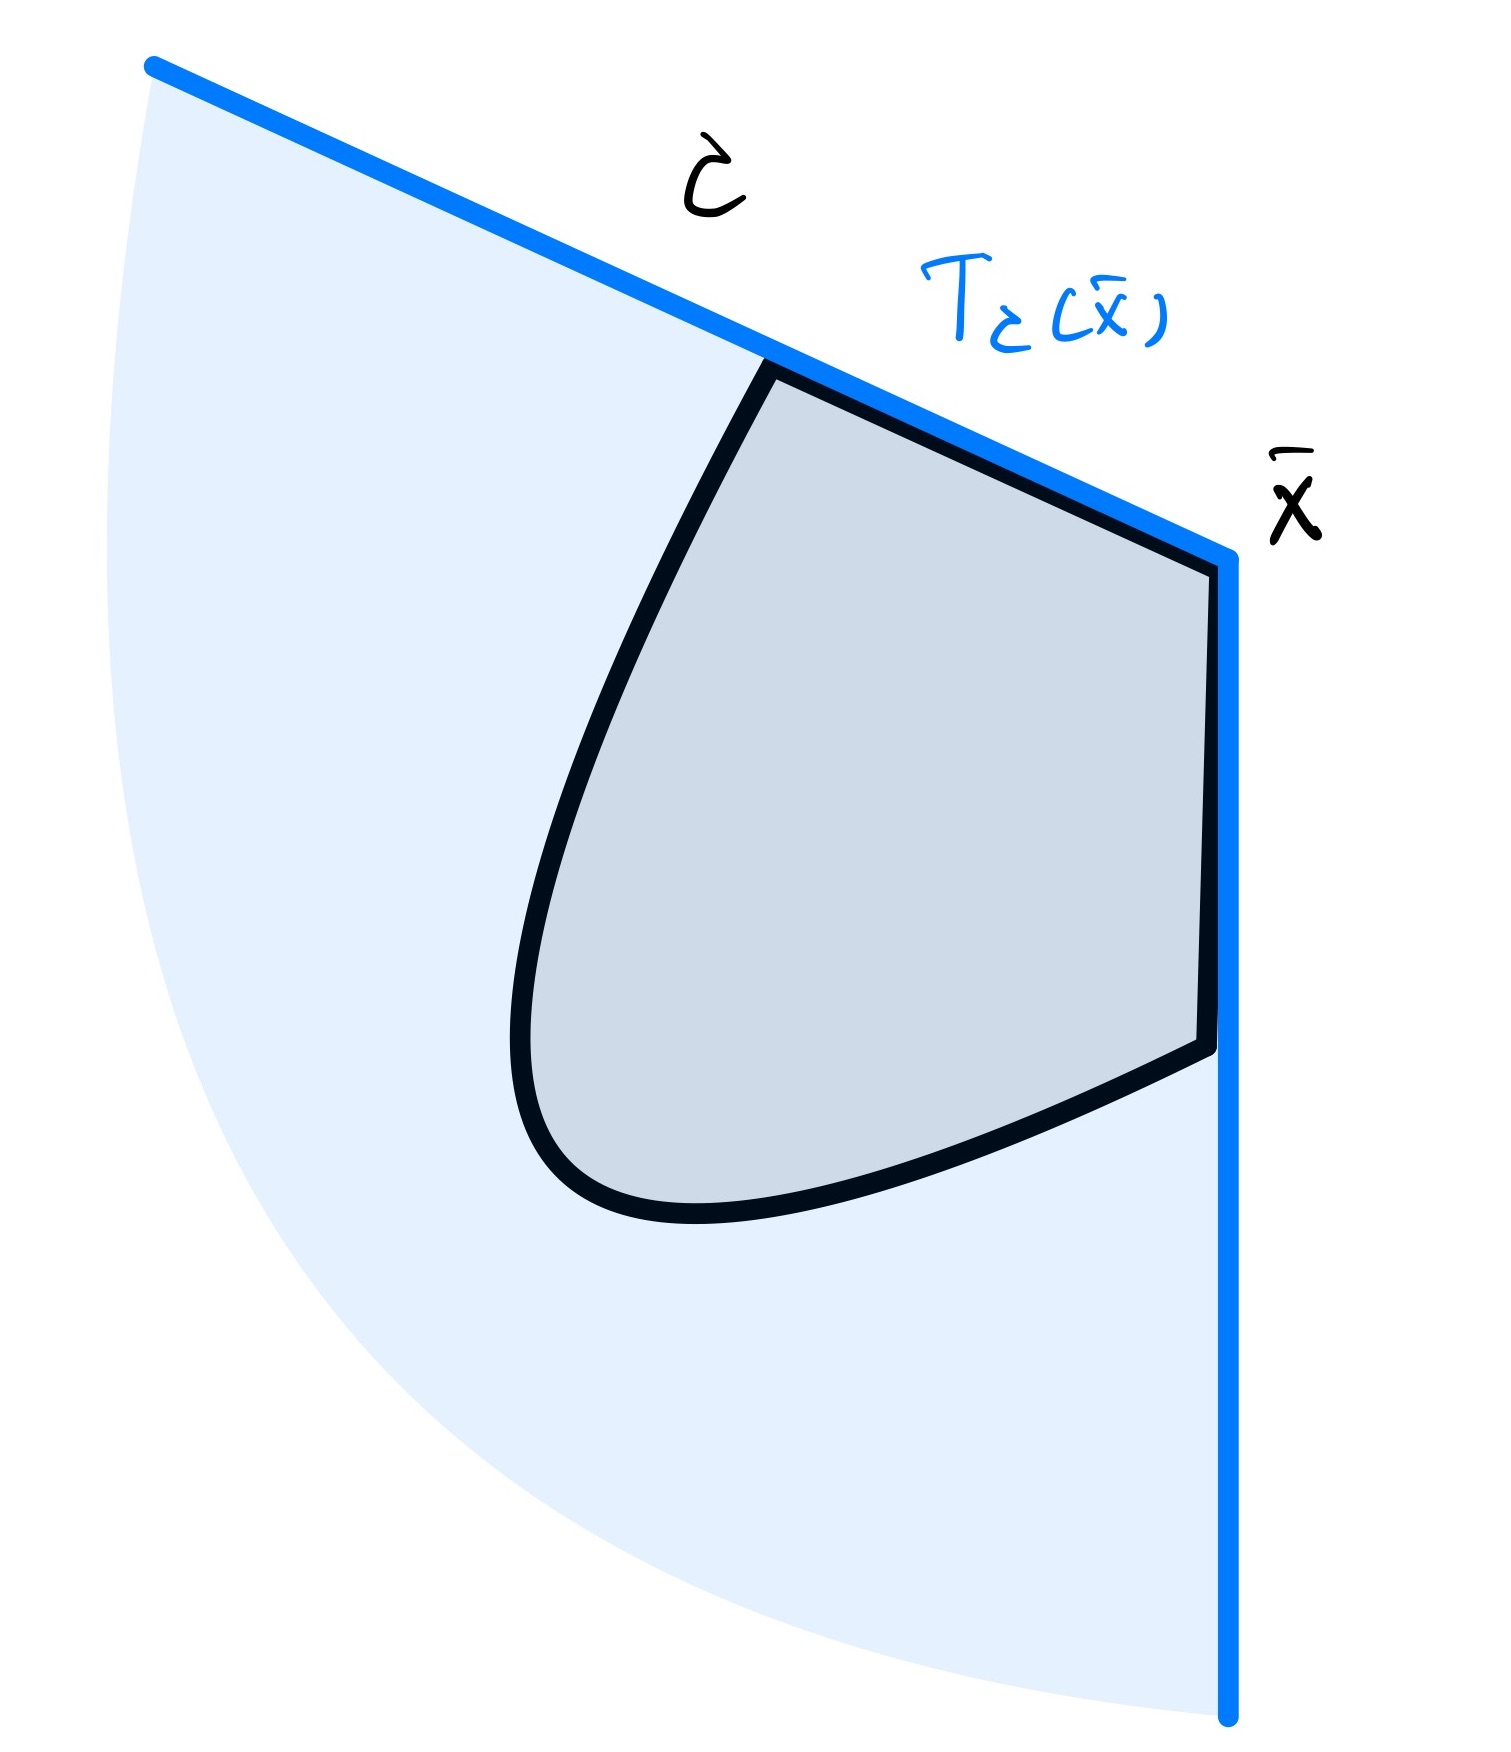
\includegraphics[keepaspectratio, scale=0.06]{figures/tangent_cone_1.jpg}
    \end{column}
    \begin{column}{0.48\textwidth}
      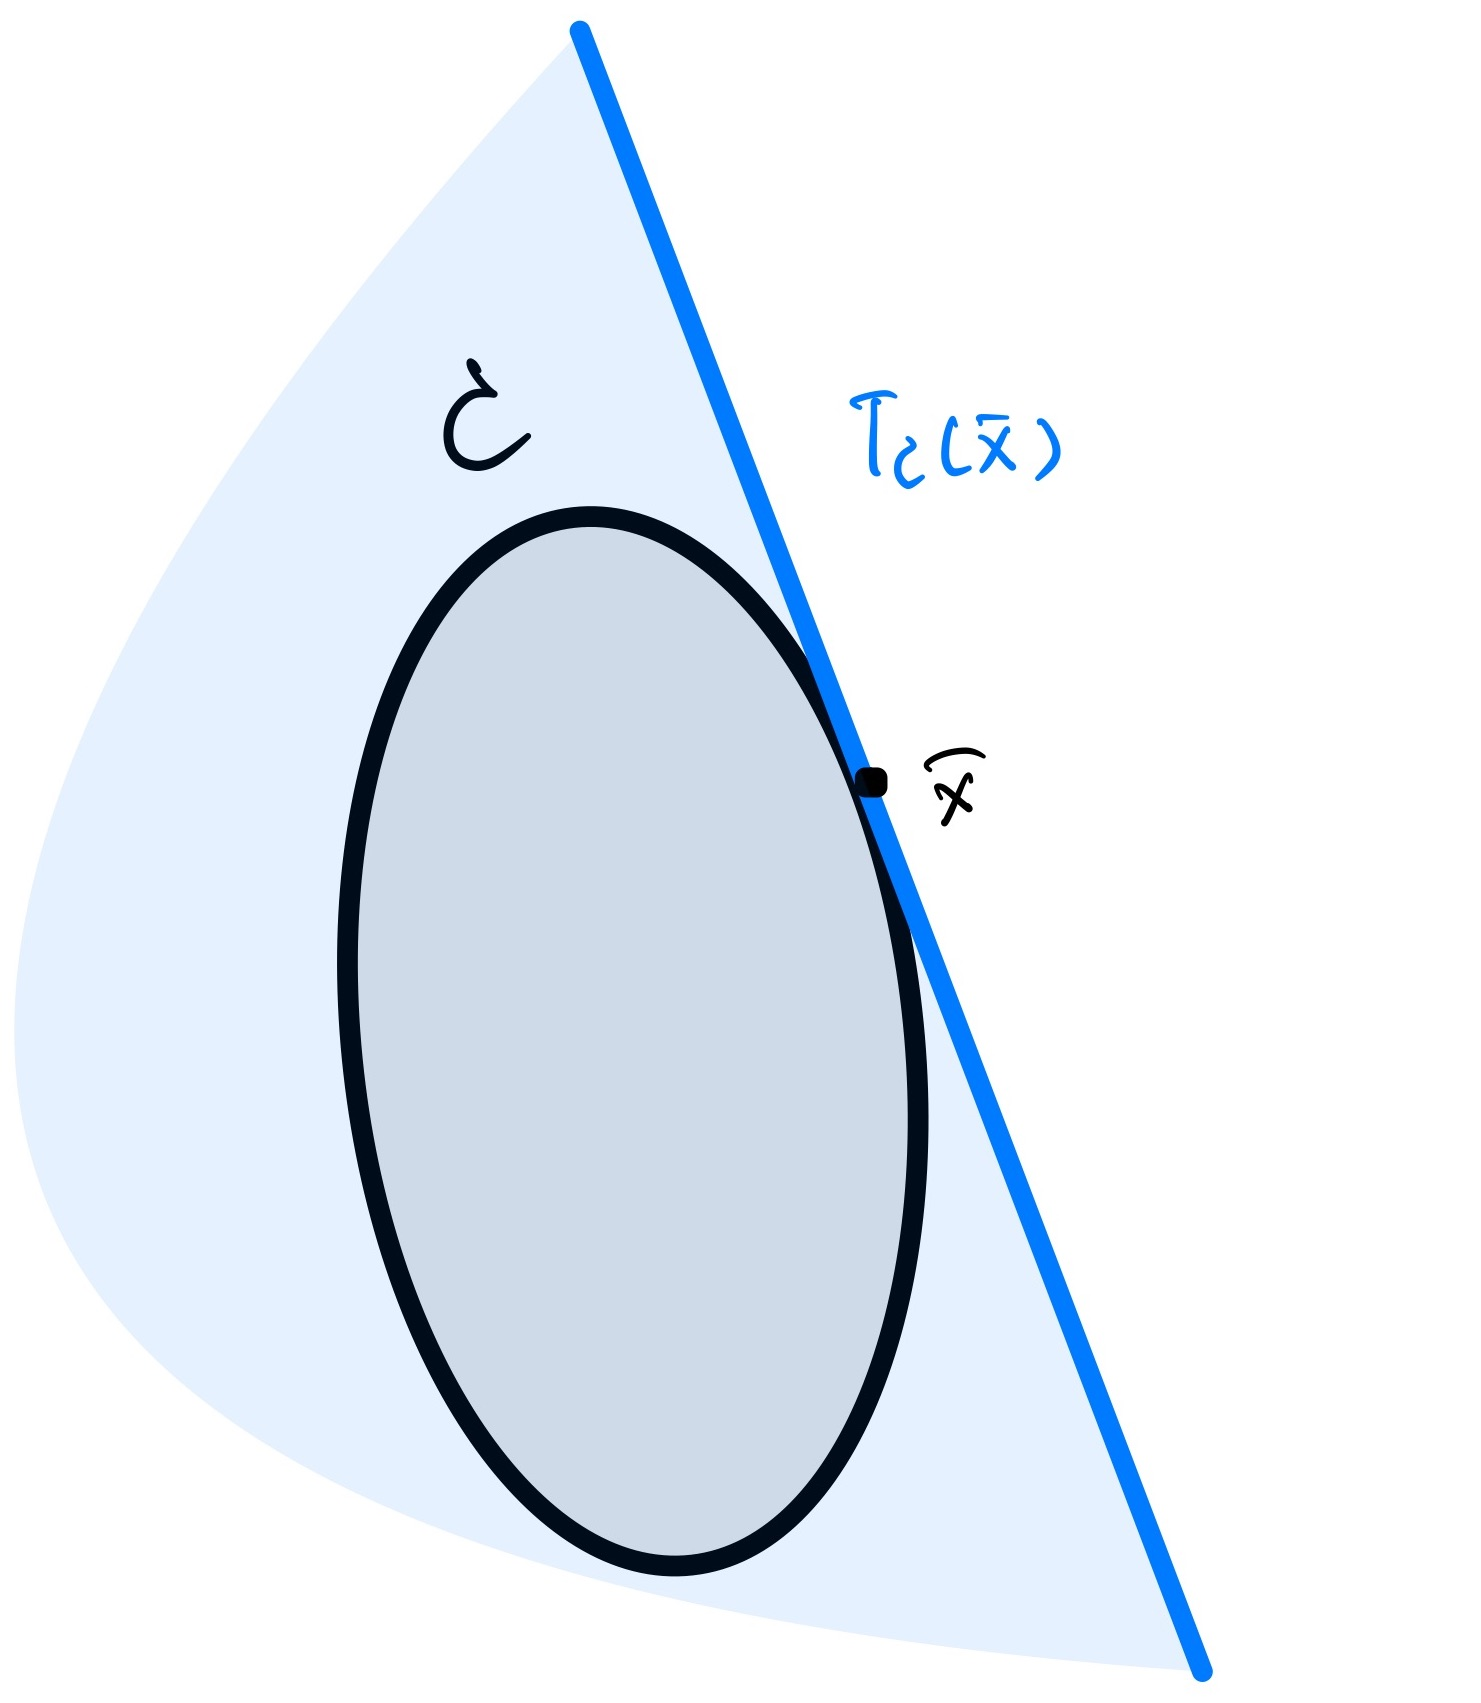
\includegraphics[keepaspectratio, scale=0.06]{figures/tangent_cone_2.jpg}
    \end{column}
  \end{columns}
\end{frame}

\section{動機づけ (Motivation) }
\begin{frame}{目次}
    \tableofcontents[currentsection]
\end{frame}

\begin{frame}{動機づけ (Motivation) (1) }

  漸近錐 (Asymptotic cones) の定義に入る前に、一般的な点列の収束について考える。

  \begin{block}{定義 3.1}
    ある点列 $\{ x_k \}$ がある点 $x$ に収束するような部分列を持つ時にこの点$x$ を点列 $\{ x_k \}$ の収積点と呼ぶ。
  \end{block}

  \begin{block}{命題 3.2}
    ある点列 $\{ x_k \}_{k \in \mathbb{N}}$ がある点 $x$ への収束することと、その点列が有界で唯一つの収積点 $x$ を持つ、ということが同値である。
  \end{block}

  一般に、$\mathbb{R} ^n$ の実ベクトル空間である点への収束性を考える場合、その集合の有界性と唯一つの収積点を持つ、ということが必要である。
\end{frame}

\begin{frame}{動機づけ (Motivation) (2) }
  \begin{alertblock}{注意}
    ここで点列が有界であることから、ボルツァーノ・ワイエルシュトラスの定理より、収束する部分列が存在することが言える。
  \end{alertblock}

\pause
  では、与えられた点列に有界性がない場合はどうすればいいのか?
\pause

  例: $D = \{(x,y) \in \mathbb{R}^2 \:|\: y=x^2\}$

  \centering
  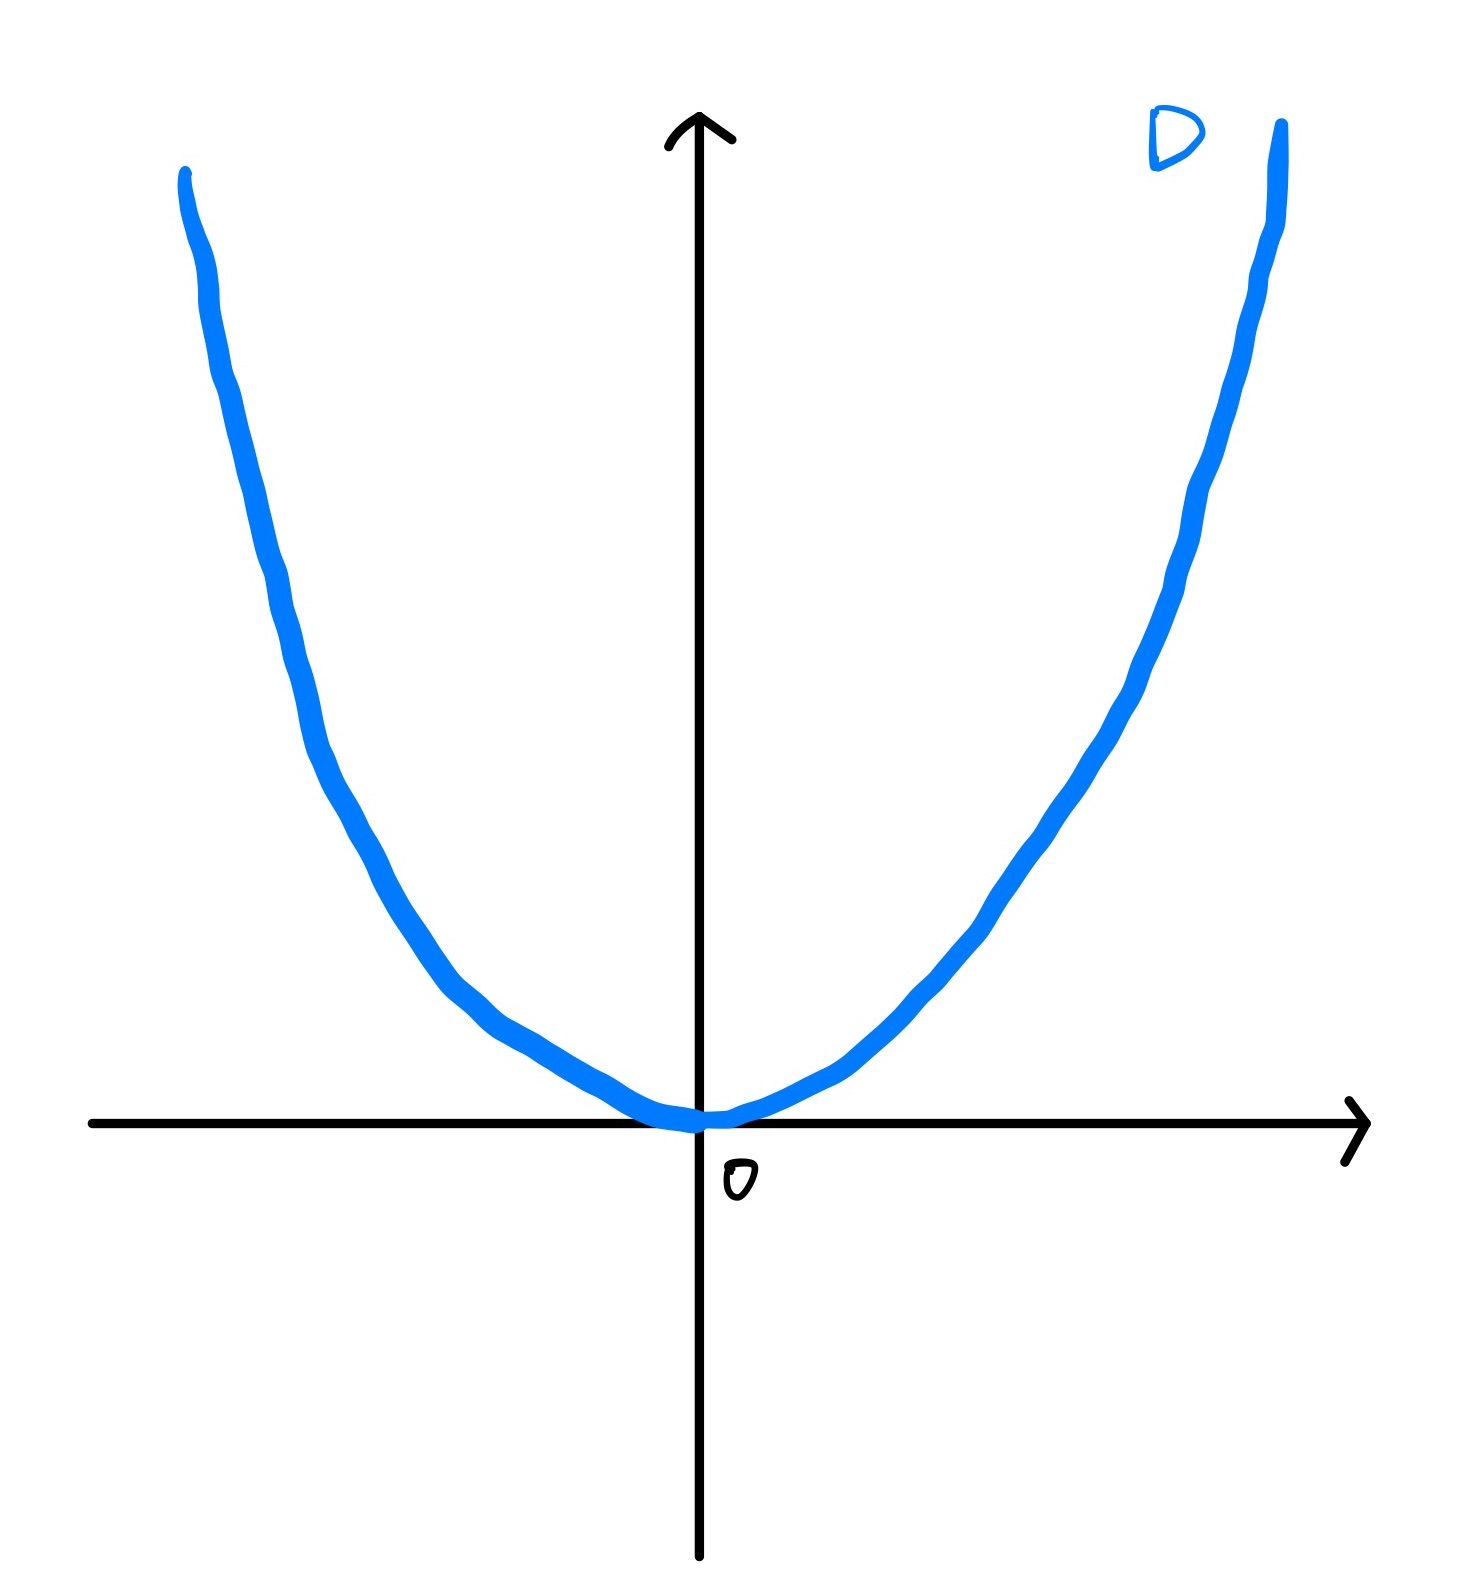
\includegraphics[keepaspectratio, scale=0.06]{figures/unbounded_example.jpg}
\end{frame}

\section{漸近錐とは (Asymptotic Cones) }
\begin{frame}{目次}
    \tableofcontents[currentsection]
\end{frame}

\begin{frame}{漸近錐とは (Asymptotic Cones) (1) }
  漸近錐の定義に入る前に改めて収束性の定義をする。
  \begin{block}{定義 4.1}
    以下の条件を満たしている時、ある点列 $\{ x_k \} \subset \mathbb{R} ^n$ が $d \in \mathbb{R} ^n$ に収束する、と定義する。

    \begin{equation}
      \exists\{ t_k \}, with\: t_k \rightarrow +\infty \:s.t.\: \lim_{k \to \infty} \frac{x_k}{t_k} = d \tag*{(2.1)}
    \end{equation}
  \end{block}
\end{frame}

\begin{frame}{漸近錐とは (Asymptotic Cones) (2) }
  漸近錐の定義をする。
  \begin{block}{定義 4.2}
    $C \subset \mathbb{R}^n$, $C \neq \varnothing$ とする。このとき$C$ の Asymptotic cone、記号で $C_\infty$ 、は点列 $\{ x_k \} \subset C$ を用いて以下のように定義する。

    \begin{equation}
      C_\infty = \{ d \in
    \mathbb{R}^n \:|\: \exists t_k \rightarrow +\infty, \exists x_k \in C \:with\: \lim_{k \to \infty} \frac{x_k}{t_k} = d \}. \notag
    \end{equation}
  \end{block}
\end{frame}

\begin{frame}{漸近錐とは (Asymptotic Cones) (3) }
  点列が有界な場合はどうなるのか?
  \begin{block}{命題 4.3}
    ある集合 $C \subset \mathbb{R}^n$ が有界であることと $C_\infty = \{0\}$ であることは必要十分である。
  \end{block}
\end{frame}

\section{今後の目標 (Next goals) }
\begin{frame}{目次}
    \tableofcontents[currentsection]
\end{frame}

\begin{frame}{今後の目標 (Next goals) }
    \begin{itemize}
    \item 漸近推の性質
    \item 漸近関数の性質
    \item 最適化問題との関係
    \end{itemize}

    これらを通して研究対象を絞っていく。
\end{frame}

\begin{frame}{最後に }
  使用しているテキストの紹介
  \begin{itemize}
  \item Asymptotic Cones and Functions in Optimization and Variational Inequalities (A.Auslender and M.Teboulle [著])
  \item 凸解析学と最適化理論 (田中謙介[著])
  \end{itemize}
\end{frame}

\end{document}
